
\section{Java-Script [R] [W]}
\subsection{Wieso Java-Script?}
Ein Stand-alone-Programm ist ein Programm, dass selbständig arbeiten kann.
Das Web-Game sollte kein Stand-alone-Programm werden, sondern im Browser erreichbar sein. Deswegen wurde JavaScript für die Programmierung am Client, sowie auch am Server ausgewählt.
Der Vorteil davon ist, dass nur eine Programmiersprache benutzt werden muss, um eine Client-Server-Architektur zu bewerkstelligen.
Außerdem besteht kein Aufwand, um Scribble-Fight spielen zu können - ein Browser ist alles, was benötigt wird.
\setauthor{Rafetseder Tobias}
\subsection{p5.js / p5.play [R]}
\label{subsection:p5js}\cite{p5js}
p5.js ist eine open-source JavaScript-Library, die für Kreation von Spielen genutzt wird.
p5.play ist eine Library für p5.js, mit der visuelle Objekte verwaltet werden können. Außerdem beinhaltet es Features wie Animation-Support,
Kollisionserkennung, sowie aber auch Funktionen für Maus- und Tastatur-Interaktionen.
p5.play ist für barrierefreies und simples Programmieren gedacht, nicht für performantes.
Es ist keine eigene Engine, und unterstützt auch keine 3D-Spiele.

\subsubsection{Einbindung}
Der einfachste Weg p5.js einzubinden, ist auf ein JavaScript File online zu verweisen.

\begin{lstlisting}
    <script 
    src="https://cdn.jsdelivr.net/npm/p5@1.4.0/lib/p5.js">
    </script>
\end{lstlisting}
Die p5.js Library kann aber auch
unter \url{https://p5js.org/download/} lokal heruntergeladen werden.
Dann kann einfach auf das lokale File verwiesen werden.

\begin{lstlisting}
    <script src="../p5.min.js"></script>
\end{lstlisting}

Jedoch muss das Projekt dann auf einem lokalen Server (z.B. mit Node.js umgesetzt) gehostet werden.

\subsubsection{Struktur eines p5.js Projekts}
Die Struktur ist sehr simpel. Im Ganzen ist es nur ein \texttt{index.html} File und ein \texttt{sketch.js} File. In dem HTML File wird die p5-Library und auch das sketch.js File eingebunden.

\begin{figure}[H]
    \centering
    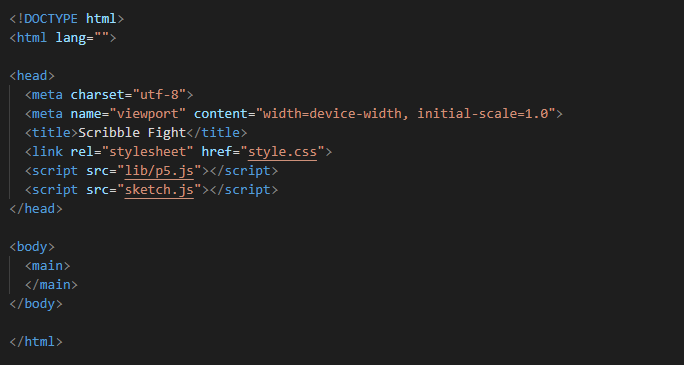
\includegraphics[scale=1]{pics/index html.PNG}
    \caption{Aufbau index.html}
\end{figure}

So können in dem sketch.js File die p5.js Methoden genutzt werden. Die wichtigsten Methoden sind die Setup- und die Draw-Methode.
Die Setup-Methode wird vor der Draw-Methode aufgerufen um das Spiel zu initialisieren. (Es wird zum Beispiel ein Canvas erstellt).
Wenn diese abgeschlossen ist, wird die Draw-Methode wiederholt aufgerufen und aktualisiert jedes mal den Bildschirm.

\begin{figure}[H]
    \centering
    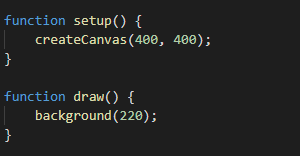
\includegraphics[scale=1]{pics/sketch.PNG}
    \caption{Simples sketch.js Beispiel}
\end{figure}

%https://www.sitepoint.com/processing-js-vs-p5-js-whats-difference/
\subsubsection{P5.js vs Processing}
p5.js ähnelt sich sehr stark mit Processing, eine Programmiersprache, die als eine stark vereinfachte Version von Java definiert werden kann.
Der Unterschied liegt darin, dass Processing eine Umgebung, basierend auf der Java Programmiersprache ist, während p5.js eine Bibliothek, basierend auf der JavaScript Programmiersprache ist.
Processing ist dafür geeignet, lokale Applikationen zu bauen, hingegen dazu kann p5.js nur im Browser ausgeführt werden.

p5.js ist sozusagen ein direkter JavaScript Port für die Processing Programmiersprache. Die Funktionen, die in Processing mit Java geschrieben werden, werden nun mit JavaScript geschrieben. \cite{p5_proc_difference}

Vorteile von p5.js:
\begin{compactitem}
    \item Die Programme, die mit p5.js umgesetzt werden, funktionieren in jedem modernen Browser (plattformunabhängig)
    \item Das Programm ist nicht nur lokal auf dem eigenen Gerät verfügbar, was das Teilen sehr viel leichter macht
    \item Es besteht die Option, den p5.js Editor im Web zu verwenden: Überhaupt kein Aufwand, um loszuprogrammieren
\end{compactitem}

Nachteile von p5.js:
\begin{compactitem}
    \item Es kann kein Stand-alone-Programm entwickelt werden, d.h. ein Browser wird benötigt
\end{compactitem}


\subsection {Node.js [R]}
Node.js ist eine plattformübergreifende Open-Source-JavaScript-Laufzeitumgebung, mit der Besonderheit, dass sie JavaScript-Code außerhalb eines Webbrowsers ausführen kann.
Sie wurde 2009 von Ryan Dahl entwickelt, einem Software-Entwickler aus Kalifornien.
Die Laufzeitumgebung wurde darauf spezialisiert, leicht skalierbare Server zu bauen. \cite{nodejs}

%https://developer.mozilla.org/en-US/docs/Learn/Server-side/Express_Nodejs/Introduction
Vorteile von Node.js: \cite{nodejs_vorteile}

\begin{compactitem}
    \item Starke Performance. Node.js ist mit Fokus auf Optimierung des Datentransport und der Skalierbarkeit bei Web-Applikationen designet worden
    \item Da mit JavaScript entwickelt wird, wird nur eine Sprache für Client und Server benötigt
    \item Da JavaScript eine relativ neue Programmiersprache ist, profitiert diese auch von Verbesserungen bei Programmiersprachen-Design (im Vergleich zu anderen Web-Server-Sprachen wie PHP oder Python)
    \item Durch den Node-Package-Manager (NPM) kann auf sehr viele Bibliotheken zugegriffen werden
    \item Es ist nicht wichtig, welches Betriebssystem verwendet wird. Node.js ist kompatibel mit Microsoft Windows, macOS, Linux, Solaris, FreeBSD, OpenBSD etc.
    \item Hinter Node.js steht eine große Entwickler-Community, die bereit ist, in Problemfällen zu helfen
\end{compactitem}


% In dem folgenden "Hello World"-Beispiel, können viele Verbindung gleichzeitig behandelt werden. Bei jeder Verbindung wird die Callback-Funktion ausgeführt, aber wenn keine Arbeit zu erledigen ist, schläft Node.js.

% \begin{figure}[H]
%     \centering
%     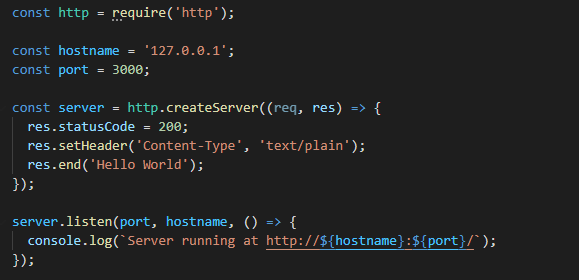
\includegraphics[scale=1]{pics/node js.PNG}
%     \caption{Sehr simpler Node.js Server}
% \end{figure}

% Man merkt den Unterschied zu den heutzutage weit verbreiteten Concurrency-Modellen, die mit OS-Threads arbeiten. Der Vorteil von Node.js hierbei ist, dass
% man sich keine Sorgen über dead-locking machen muss, da fast keine Node.js Funktion direkte I/O Operationen durchführt. Also ist der ganze Prozess so gut wie nie blockiert, ausser
% wenn synchrone Methoden der Node.js Standard Library benutzt wird.

\subsubsection{Node Package Manager}\label{NPM}
Neben Node.js an sich, ist NPM (Node Package Manager) das wichtigste Werkzeug für Node.js Applikationen. Mit NPM können alle Packages, die das Projekt benötigt, geholt werden.
Es ist möglich, alle Packages einzeln zu holen, jedoch wird in der Praxis immer ein package.json-File benutzt. In diesem File stehen alle Dependencies für jedes JavaScript Package,
das benötigt wird, sowie auch Meta-Daten zu dem Node.js Projekt. \cite{node_environment}  \\
Erstellt wird dieses mit dem Befehl \texttt{npm init}. Es spielt jedoch eine Rolle, wo dieser Befehl ausgeführt wird, also muss darauf geachtet werden, dass der Befehl in dem Verzeichnis ausgeführt wird, in dem das Projekt erstellt werden soll.
Die Struktur eines package.json-Files sieht wie folgt aus:
\begin{figure}[H]
    \centering
    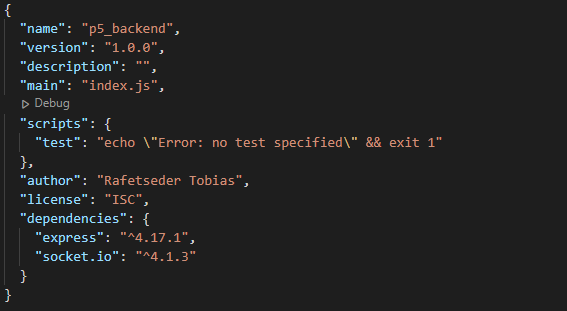
\includegraphics[scale=1]{pics/package json.PNG}
    \caption{Package.json des Scribble-Fight Backends}
\end{figure}

\subsubsection{Express}
Express ist das am meisten verbreitetste Node-Web-Framework und ist auch die Basis für andere Node-Web-Frameworks. Die Hauptverantwortung
von Express ist das Bereitstellen von Server-Logik, wie zum Beispiel das Schreiben von Handlers für Requests mit unterschiedlichen Http-Request-Methoden (GET, POST, PUT etc.) auf unterschiedlichen URL-Pfaden. \cite{node_environment} \\
Express wird mit dem Node-Package-Manager mit \texttt{npm install express} installiert. Befindet sich der Benutzer in
einem Verzeichnis, das ein package.json-File beinhlatet, bei dem Express als Dependency hinzugefügt wurde, dann reicht \texttt{npm install} für die Installation.

\begin{figure}[H]
    \centering
    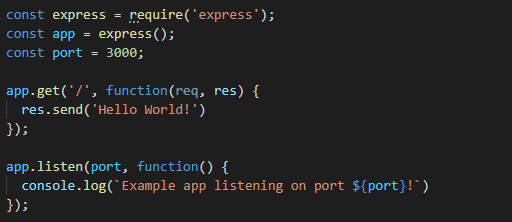
\includegraphics[scale=1]{pics/Express.PNG}
    \caption{Simpler Web Server mit Express}
\end{figure}

\subsection{Socket IO [R]}

Socket.IO ist eine Library, die eine bidirektionale Echt-Zeit Verbindung zwischen Server und Client ermöglicht. Sie baut auf das WebSocket-Protokoll auf, das bedeutet es gibt neben den WebSocket-Funktionen auch noch additionale Funktionen wie zum Beispiel eine automatische Wiederverbindung.

Um dem Client des Spiel im Browser eine bidirektionale Echt-Zeit Kommunikation mit dem Server bereitzustellen, wurde benutzt:
\begin{compactitem}
    \item Ein Node.js Server inklusive SocketIO Package
    \item Eine JavaScript Client Library von SocketIO (Es bestehen auch einige andere Client Implementationen für Sprachen wie Java, C++, Python, etc.)
\end{compactitem}

Socket.IO funktioniert so, dass der Client, falls möglich, eine SocketIO-Verbindung mit dem Server herstellt.
Ist keine Verbindung möglich, setzt der Client einen HTTP-long polling-Request ab, also ein Request an den Server, der diesen so lange offen hält, bis neue Daten geschickt werden können. \cite{httpLongPolling} \\
Am Client sieht die Syntax für die JavaScript-Library so aus:

\begin{figure}[H]
    \centering
    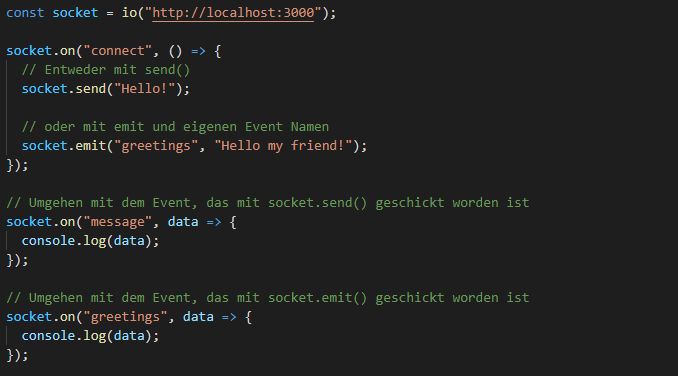
\includegraphics[scale=1]{pics/SocketIO_client.PNG}
    \caption{Socket.IO Client Beispiel}
    \label{tech:socketioclient}
\end{figure}

Damit der Server die Verbindung annehmen kann, müssen folgende Kriterien erfüllt sein:
\begin{compactitem}
    \item Der Browser unterstützt WebSocket
    \item Die Verbindung wird nicht von Elementen wie Firewall gestört
\end{compactitem}
Die API ist auf der Server-Seite dem Client sehr ähnlich, es existiert auch wieder ein \texttt{socket} Objekt, welches von der EventEmitter Klasse von Node.js erbt. Ein Beispiel für den serverseitigen Code, der zu dem Client-Code von Abbildung \ref{tech:socketioclient} gehört:

\begin{figure}[H]
    \centering
    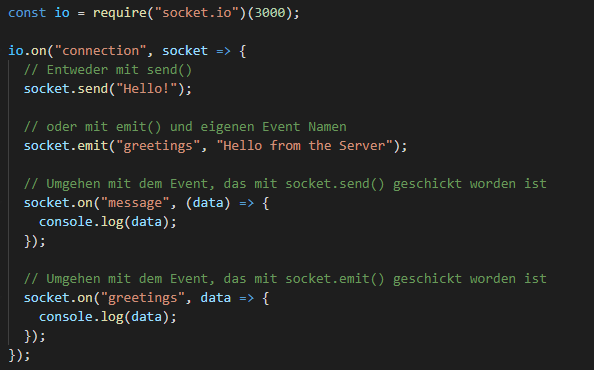
\includegraphics[scale=1]{pics/SocketIO_server.PNG}
    \caption{Socket.IO Server Beispiel}
\end{figure}


\subsubsection{Unterschied Socket.IO zu WebSocket}
Socket.IO ist keine WebSocket Implementation. Auch wenn Socket.IO WebSocket als Transportmittel benutzt, werden bei jedem Paket zusätzliche Metadaten angehängt. Das ist auch der Grund, warum
ein Socket.IO Client keine Verbindung mit einem schlichten WebSocket Server herstellen kann, und umgekehrt.
Das heißt, Socket.IO ist ein Wrapper rund um die WebSocket API. \cite{socketio}


\setauthor{Weinzierl Ben}
\subsection{qrcode.js [W]}
Ein QR-Code ist ein Matrix-Barcode welcher meistens auf eine bestimmte URL verweist. Die Bezeichnung QR steht für Quick Response,
also schnelle Antwort. Für die Codierung verwendet der QR-Code 4 Methoden: Numerisch, Alphanumerisch, Byte/Bit und Kanji.
Besonders populär wurde das QR-Code System dank seiner
schnellen Lesbarkeit und seiner erhöhten Speicherkapazität im Vergleich zu den
damalig verwendeten UPC Barcodes(sh. Abbildung 10). Anwendungsfälle für QR-Codes sind Produkt-Tracking, Item-Identifikation, Dokumentenmanagement, etc. .
Ein QR-Code besteht aus schwarzen Quadraten welche in einem großen Quadrat arrangiert werden(sh. Abbildung 9).
Dieser kann einfach von einer Kamera oder ähnlichem gescannt und ausgewertet werden.
Das QR-Code-System wurde von Masahiro Hara von der japanischen Autofirma Denso Wave entwickelt.
Das Design basiert auf den schwarzen und weißen Spielfiguren des Go-Spiels.
Ursprünglich wurde das System zum tracken von Fahrzeugen während der Herstellung verwendet.
Heutzutage werden QR-Codes vor allem im Werbebereich verwendet. Oft wird der
potenzielle Kunde dazu eingeladen  sein Smartphone herauszuholen und einfach den QR-Code zu Scannen um
ihn dann auf der Webseite Produkte anzubieten.

\begin{figure}[H]
    \centering
    
\includegraphics[scale=1]{pics/googleQR.png}
    \caption{QR-Code zu www.google.com}
\end{figure}

\begin{figure}[H]
    \centering
    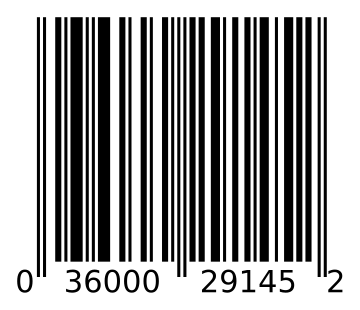
\includegraphics[scale=0.8]{pics/UPCBarcode.png}
    \caption{UPC Barcode}
\end{figure}


Hier ist ein einfaches Beispiel wie qrcode.js in eine Webseite eingefügt werden kann.
Dieser verweist auf https://www.google.com. Wichtig ist hierbei anzumerken, dass dafür die qrcode.js Javascript Bibliothek einzubinden ist.
Diese kann unter http://davidshimjs.github.io/qrcodejs/ gedownloaded werden.
\begin{lstlisting}[language=html,caption=QR-Code Demo,label=lst:tech:gaussianBlur]
<html lang="en">

    <head>
        <meta charset="UTF-8">
        <meta http-equiv="X-UA-Compatible" content="IE=edge">
        <meta name="viewport" content="width=device-width, initial-scale=1.0">
        <title>QR-Demo</title>
        <script src="qrcode.min.js"></script>
    </head>
    
    <body>
        <div id="qrcode"></div>
        <script type="text/javascript">
            new QRCode(document.getElementById("qrcode"), "https://www.google.com");
        </script>
    </body>
    
</html>
\end{lstlisting}

Bei qrcode.js können auch weitere Parameter für den QR-Code gesetzt werden. Es können
Beispielsweise Farbe, Größe, etc. verändert werden.

\begin{lstlisting}[language=html,caption=QR-Code Demo 2,label=lst:tech:gaussianBlur]
    var qrcode = new QRCode(document.getElementById("qrcode"), {
            text: "www.google.com",
            width: 512,
            height: 512,
            colorDark: "#B3FF78",
            colorLight: "#F677FF",
            correctLevel: QRCode.CorrectLevel.H
        });
\end{lstlisting}
Das Resultat dieser Veränderung sieht so aus:
\begin{figure}[H]
    \centering
    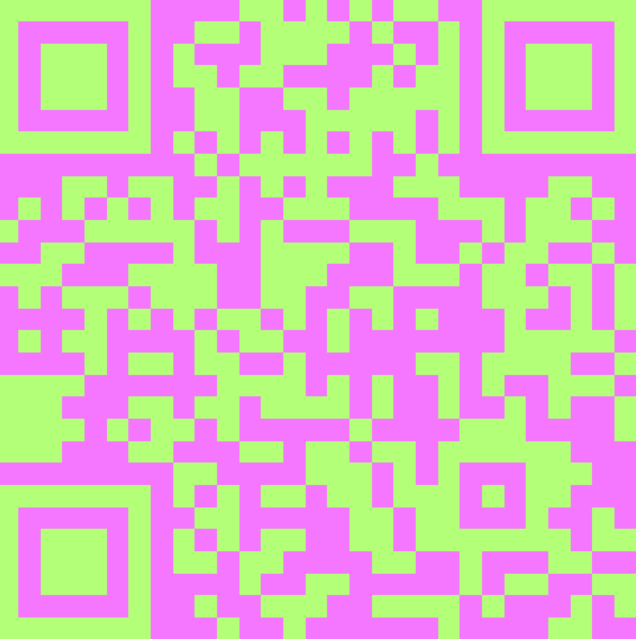
\includegraphics[scale=0.7]{pics/fancyQR.png}
    \caption{Personalisierter QR-Code}
\end{figure}

Bei dieser Arbeit wurde der QR-Code verwendet mit dem Handy zugriff auf den Mapscanner und
das Hochladen der Zeichnung zu gewährleisten.

\subsection{Chart.js [W]}
Chart.js ist eine Open-Source JavaScript Bibliothek welche es ermöglicht einfach und schnell Diagramme
in eine Webseite einzubauen. Die Bibliothek kann entweder mit dem Shell-Befehl \textit{npm i chart.js} eingebunden werden oder via Github unter
\textit{https://github.com/chartjs/Chart.js} gedownloaded werden. Chart.js stellt einem sehr
viele Möglichkeiten zur Verfügung um die Diagramme zu personalisieren.
Ihre Bibliothek hat alle denkbaren Diagrammtypen (Balkendiagramm, Kuchendiagramm, Liniendiagramm, ..., sh. Abbildung 12-14)
Eine einfaches Beispiel für ein Balkendiagramm sieht so aus:
\begin{lstlisting}[language=html,caption=Balkendiagramm HTML Code,label=lst:tech:gaussianBlur]
<html lang="en">

    <head>
        <meta charset="UTF-8">
        <meta http-equiv="X-UA-Compatible" content="IE=edge">
        <meta name="viewport" content="width=device-width, initial-scale=1.0">
        <title>QR-Demo</title>
        <script src="chart.min.js"></script>
    </head>

    <body>
        <canvas id="myChart" width="200" height="200"></canvas>
        <script>
            const ctx = document.getElementById('myChart').getContext('2d');
            const myChart = new Chart(ctx, {
                type: 'bar',
                data: {
                    labels: ['Red', 'Blue', 'Yellow', 'Green', 'Purple', 'Orange'],
                    datasets: [{
                        label: '# of Votes',
                        data: [12, 19, 3, 5, 2, 3],
                        backgroundColor: [
                            'rgba(255, 99, 132, 0.2)',
                            'rgba(54, 162, 235, 0.2)',
                            'rgba(255, 206, 86, 0.2)',
                            'rgba(75, 192, 192, 0.2)',
                            'rgba(153, 102, 255, 0.2)',
                            'rgba(255, 159, 64, 0.2)'
                        ],
                        borderColor: [
                            'rgba(255, 99, 132, 1)',
                            'rgba(54, 162, 235, 1)',
                            'rgba(255, 206, 86, 1)',
                            'rgba(75, 192, 192, 1)',
                            'rgba(153, 102, 255, 1)',
                            'rgba(255, 159, 64, 1)'
                        ],
                        borderWidth: 1
                    }]
                },
                options: {
                    scales: {
                        y: {
                            beginAtZero: true
                        }
                        
                    }
                }
            });
        </script>

    </body>

</html>
\end{lstlisting}
Die Parameter die hier verwendet wurden sind type, welcher den Typ des Diagramms angibt,
in diesem Fall bar für Balkendiagramm, data, welcher ein JSON Object mit weiteren Parametern ist.
Zum Schluss wurde mit options.scales.y.beginAtZero noch festgelegt, dass der Graph bei 0 beginnen soll.

Mit Veränderung des type Parameters können sehr einfach die Diagrammtypen verändert werden:
\begin{figure}[H]
    \centering
    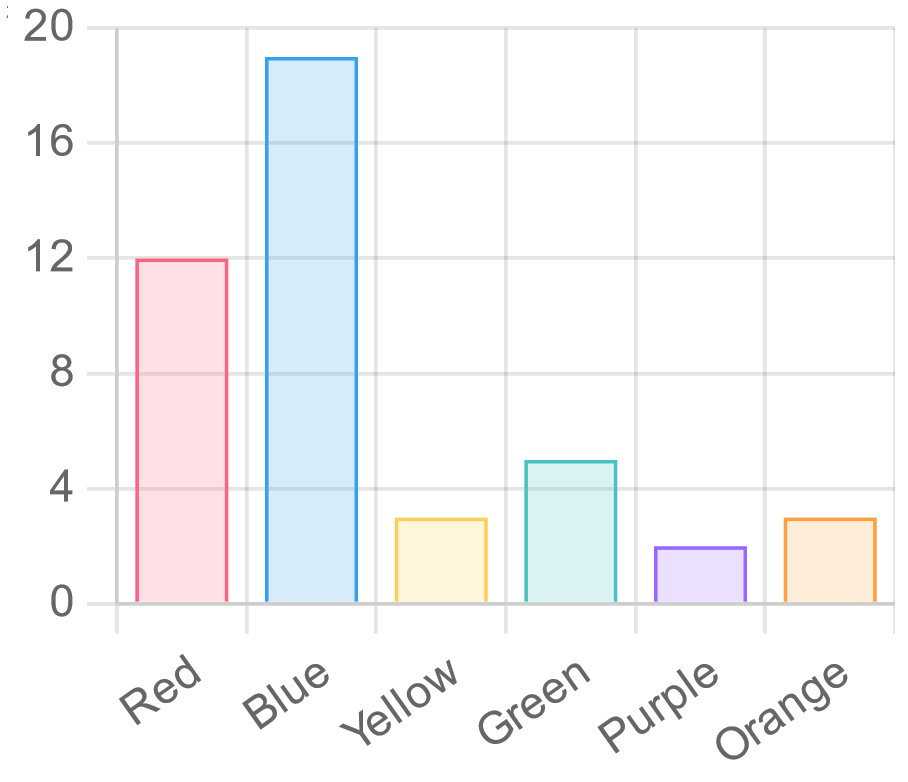
\includegraphics[scale=0.3]{pics/barChart.png}
    \caption{Barchart}
\end{figure}
\begin{figure}[H]
    \centering
    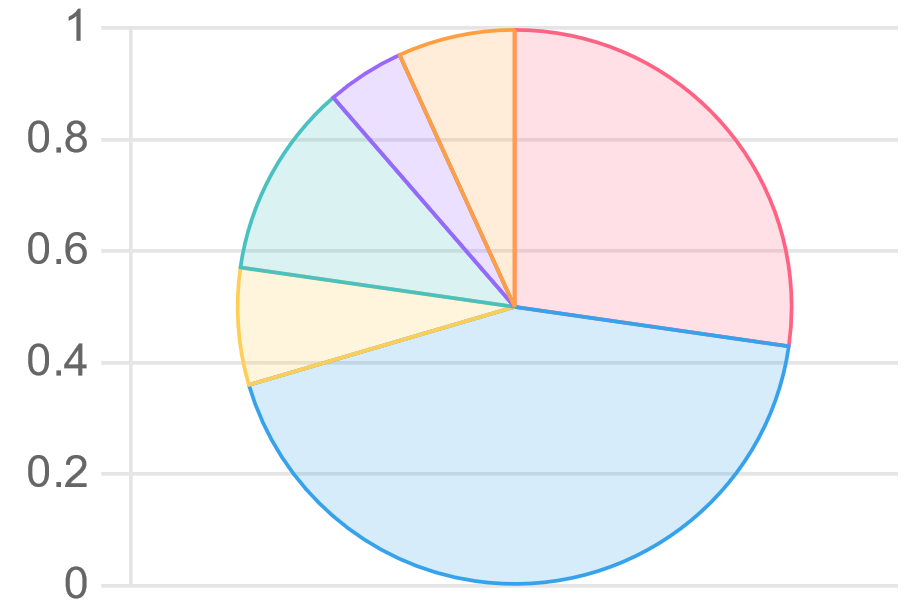
\includegraphics[scale=0.3]{pics/pieChart.png}
    \caption{Piechart}
\end{figure}
\begin{figure}[H]
    \centering
    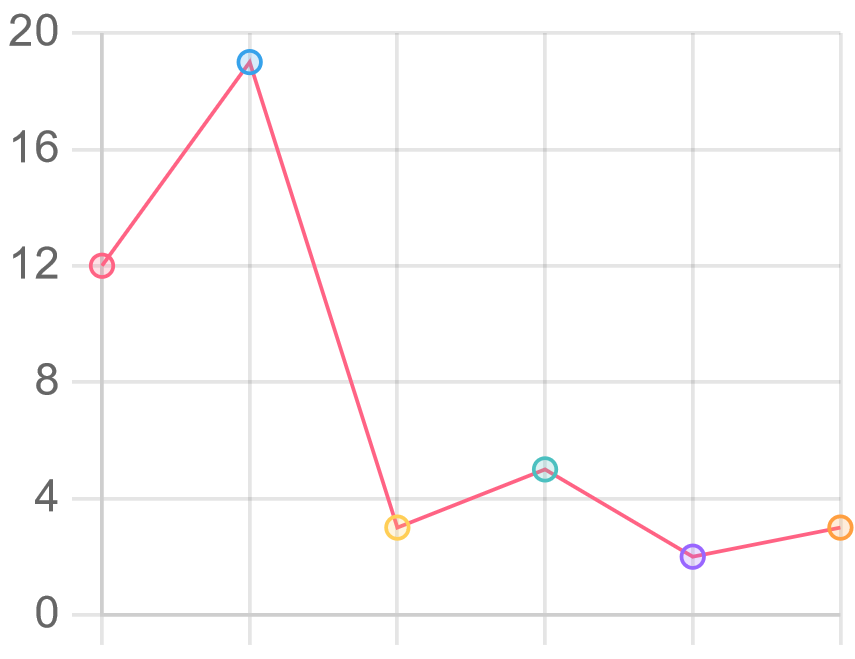
\includegraphics[scale=0.3]{pics/lineChart.png}
    \caption{Linechart}
\end{figure}

Chart.js stellt noch viele weitere hilfreiche Optionen zur Verfügung. Wird
zum Beispiel ein logarithmischer Graph benötigt kann dies mit options.scales.myscale.type = "logarithmic" eingestellt werden

\begin{figure}[H]
    \centering
    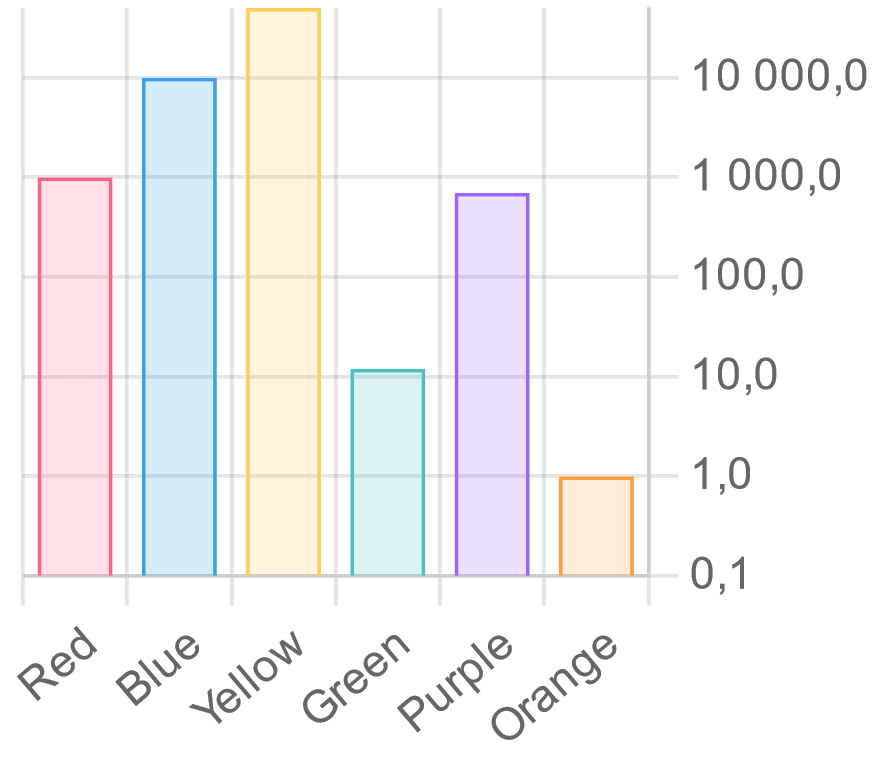
\includegraphics[scale=0.3]{pics/logChart.png}
    \caption{Logarithmisch an der Y-Achse}
\end{figure}
\begin{figure}[H]
    \centering
    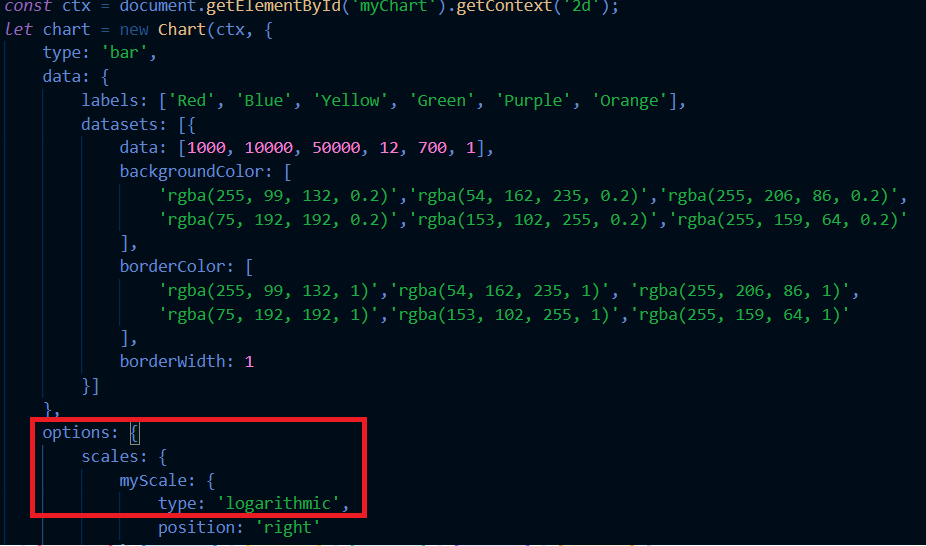
\includegraphics[scale=0.7]{pics/logCode.png}
    \caption{Code}
\end{figure}


Weitere hilfreiche Einsellungen sind:
\begin{compactitem}
    \item yAxis/xAxis: Konfigurierung der Y- und X-Achse
    \item label: Die Bezeichnung für den Datensatz, die in der Legende erscheint.
    \item color: Weißt einem Label eine bestimmte Farbe zu
    \item datasets.data: Weißt einem label Daten zu
    \item layout: Konfigurierung des Layouts des Diagramms
    \item ...
\end{compactitem}

Ist es notwendig ein Diagramm zu updaten kann dies mit diesen Funktionen umgesetzt werden. Zum hinzufügen
von Daten muss als Parameter das Diagramm, der Name des Labels und die Daten mitgegeben werden. Zum entfernen wird nur das Chart benötigt.
\begin{figure}[H]
    \centering
    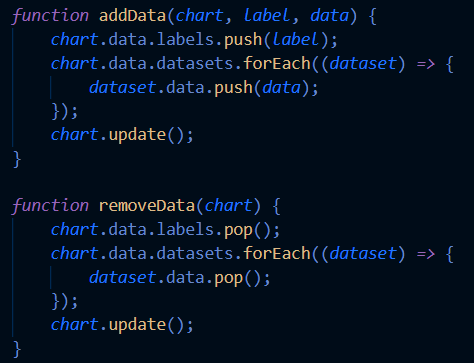
\includegraphics[scale=1]{pics/updateChart.png}
    \caption{Code zum updaten eines Diagramms}
\end{figure}




\section{Deployment [R]}
Das Scribble-Fight Browser-Game wurde in die Leocloud, ein Cloud-System der HTL-Leonding, unter \url{https://student.cloud.htl-leonding.ac.at/t.rafetseder/scribble-fight/} deployed.
Zuerst wurde mithilfe von der Docker-Technologie ein Docker-Image erstellt und auf die Leocloud hochgeladen. Das Deployment wurde dann mithilfe von Kubernetes umgesetzt.
Nähere Beschreibung zu Docker und Kubernetes folgt in den nächsten Kapiteln.
\subsection{Docker [R]} \label{tech:docker}
Die Software Docker ist eine Technologie zum Containerisieren von Prozessen, die dann unabhängig voneinander und isoliert ausgeführt werden können. Diese isolierte Prozesse werden Container genannt.
Durch die Unabhängigkeit, die dadurch entsteht, wird die Infrastruktur besser genutzt und auch die Sicherheit bewahrt, die sich aus der Arbeit mit voneinander getrennten System ergibt.
Docker arbeitet mit einem Image-basierten Bereitstellungsmodell. Dieses wird gerne bei Containertools verwendet, da Applikationen mit all deren Dependencies, egal in welcher Umgebung, genutzt werden können. \cite{docker} \\
Vorteile von Docker: \cite{docker_vorteile}
\begin{compactitem}
    \item Wenn der Benutzer einmal seine containerisierte Applikation getestet hat, kann er sich sicher sein, dass die Applikation auf jeder anderen Umgebung, auf dem Docker installiert ist, auch funktioniert
    \item Alle Docker Container sind komplett voneinander unabhängig
    \item Falls Skalierung notwendig ist, können schnell neue Container erstellt werden
    \item Im Gegensatz zu virtuellen Maschinen beinhalten Container keine eigenen Betriebssysteme, deshalb können sie schneller erstellt und auch schneller gestartet werden
\end{compactitem}

Wichtige Begriffe, im Zusammenhang mit Docker:

\begin{compactitem}
    \item Image: Speicherabbild eines Containers
    \item Container: aktive Instanz eines Images
    \item Dockerfile: eine Textdatei, die den Aufbau des Images beschreibt
    \item Registry: Unter Registry wird eine Ansammlung gleicher Images mit verschiedenen Tags verstanden, meistens Versionen
\end{compactitem}

\subsubsection{Docker Architektur}
Die Docker Architektur ist eine Server-Client Architektur. Der Docker Client kommuniziert mit dem Docker Daemon (Ein Hintergrundsprozess), der dann Docker Container z.B. baut und ausführt.
Dieser Docker Daemon kann lokal installiert sein, aber der Client kann sich auch mit einem Daemon Remote verbinden. \cite{docker_architektur}

\begin{figure}[H]
    \centering
    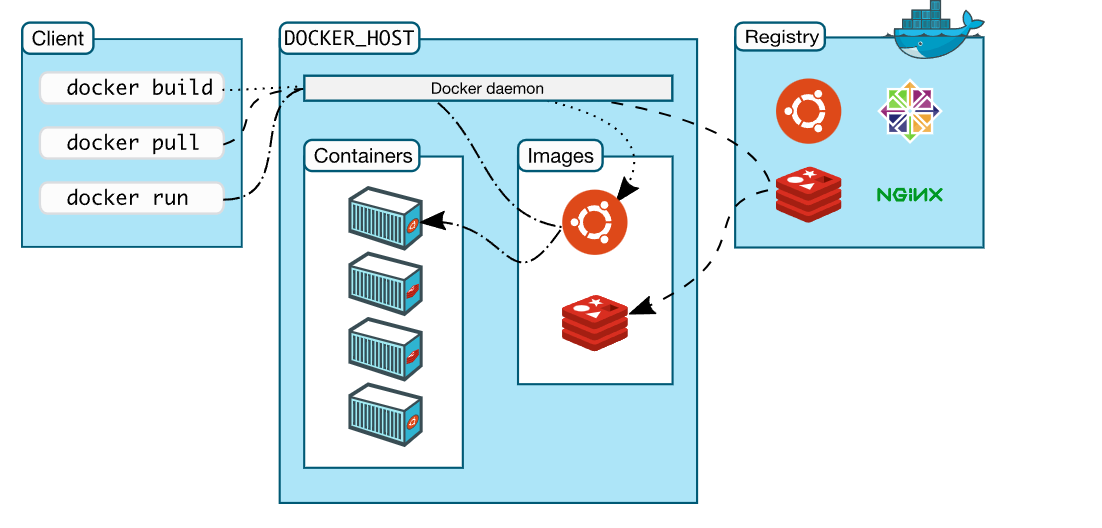
\includegraphics[scale=0.6]{pics/docker architecture.PNG}
    \caption{Veranschaulichung Docker Architektur}
\end{figure}


\subsection{Kubernetes [R]}
Kubernetes ist eine Open-Source-Plattform, die dafür genutzt wird, containerisierte Applikationen und Services zu verwalten (z.B. Computer-, Netzwerk und Speicherinfrastruktur von Containern)
Das Kubernetes-Projekt ist 2014 als Open-Source Projekt in die Welt gerufen worden.

Kubernetes hat mehrere Funktionen, zum Beispiel ist Kubernetes:
\begin{compactitem}
    \item eine Containerplattform
    \item eine Microservices-Plattform
    \item eine Cloud-Plattform
\end{compactitem}
\cite{kubernetes}

In dieser Diplomarbeit wird Kubernetes benutzt, um ein mit Docker gebautes Images des Web-Servers und des Clients auf ein Cloudsystem zu deployen. Näheres zur Umsetzung wird in Kapitel \ref{impl:Deployment} beschrieben


\newpage
\section{Python [H]}
Die Programmiersprache Python
fand in unserer Arbeit zwei Haupteinsatzgebiete. \\
Erstens zur Erkennung des Blatt Papiers und der Umwandlung der Zeichnung in eine spielbare Map
und zweitens, um die Künstliche Intelligenz zu erschaffen. \\
Die kostenlosen Bibliotheken, welche wir dabei in Verwendung haben, werden im folgenden gelistet und näher
erklärt.
Der Vorteil von Python, und auch der Grund warum die Sprache den Einsatz in dieser Arbeit fand, ist, weil
viele Hilfestellungen und Bibliotheken verfügbar sind.
\setauthor{Himmetsberger Jonas}

\subsection{Flask [H]}
Flask ist das am wohl häufigste verwendete Python Web-Framework. Somit gibt es viele Tutorials,
Tools und Bibliotheken. Diese sind sehr gut bis gut dokumentiert und teilweise geprüft.
Aus diesen Gründen haben wir den Teil der Bild- und Maperkennung, welche
als Webanwendung funktioniert, mittels Flask umgesetzt. In Kombination mit Flask-SocketIO werden Bilder von der Webcam
in Echtzeit direkt an den Server geschickt, welcher dann via OpenCV2 Informationen aus dem Bild
generiert. Genau wie bei SocketIO in JavaScript, agiert Flask-SocketIO als bidirektionale
Kommunikation zwischen Server und Client. Die extrem geringe Latenzzeit, welche dabei auftritt,
ist wichtig um eine flüssige Verarbeitung der Bilder zu gewährleisten.

\subsection{OpenCV2 [H]}
Open ``Computer Vision'' (CV) wurde in unserem Kontext als Python Bibliothek verwendet. OpenCV verfügt über eine
breitgefächerte Auswahl an Bildverarbeitungs-Algorithmen.
Folgende wurden bei der Maperkennung eingesetzt:
\begin{compactitem}
    \item Resizing
    \item Farbraumkonvertierung
    \item Weichzeichnung
    \begin{compactitem}
        \item Median-Blur
        \item Gaussian-Blur
    \end{compactitem}
    \item adaptive Schwellenwertbildung von Pixelwerten
    \item Konvertierung eines Zahlen Arrays in eine ``.png'' datei
\end{compactitem}
Auf die Funktionsweise dieser Algorithmen wird im Folgenden (\ref{maai:alogs}) genauer eingegangen.
\\
Um zum Beispiel ein beliebiges Bild unscharf zu zeichnen würde man so vorgehen:
\\

\begin{lstlisting}[language=Python,caption=OpenCV Demo,label=lst:tech:gaussianBlur]
    # Dieses kurze Programm soll ein Bild in Python mittels Open Computer Vision weichzeichnen
    
    # Importieren der gebrauchten Bibliothek
    import cv2
    import numpy
    
    # Bild einlesen
    source = cv2.imread('./Pfad/zum/Bild.png', cv2.IMREAD_UNCHANGED)
    
    # Das Quell-Bild wird nun unscharf gezeichnet
    destination = cv2.GaussianBlur(source,(5,5),cv2.BORDER_DEFAULT)

    # Anzeigen von dem Quellbild und dem bearbeiteten Bild 
    cv2.imshow('Weichzeichnung',numpy.hstack((source, destination)))

    # warten, bis eine Taste gedrueckt wurde
    cv2.waitKey(0) 

    # Alle Fenster, welche die Bilder anzeigen, werden geschlossen
    cv2.destroyAllWindows() 
\end{lstlisting}

%Quelle: https://opencv.org/

\subsection{PIL [H]}
PIL (Python Image Library) ist, wie Flask und OpenCV2, eine kostenlose Zusatzbibliothek für Python.
PIL wird verwendet, um Bilder zu speichern und einzelne Pixel zu manipulieren. Dabei unterstützt PIL diese
Dateiformate: PPM, PNG, JPEG, GIF, TIFF, und BMP. Pixel manipulation bedeutet, dass jeder Pixel auf einem
Input Bild angepasst werden kann. Beispiele hierfür sind zum Beispiel das Aufhellen oder Abdunkeln von
Bildern oder das Anpassen der Sättigung. Auch Kontrast- oder Schärfeeinstellungen können mit
Pixelmanipulation erzielt werden. Dafür werden meistens Matrizen und/oder Formeln pro Pixel verwendet, um
deren Farbwerte anzupassen
\\



\begin{lstlisting}[language=Python,caption=PIL Demo,label=lst:tech:PIL]
    # import
    from PIL import Image, ImageFilter  

    source = Image.open("file.ppm") # Load an image from the file system.
    destination = source.filter(ImageFilter.BLUR) # Blur the image.

    # Display both images.
    source.show() 
    destination.show()
\end{lstlisting}



\subsection{TensorFlow und Keras [H]}
TensorFlow ist eine Python Bibliothek, welche beim erstellen von Projekten, die maschinelles Lernen
in irgend einer Art und Weise eingebunden haben, extrem unterstütz.
Wie der Name schon vermuten lässt, basiert TensorFlow auf zwei Grundlagen: Tensoren und Graphen (Flow
vom Wort dataflow). \\
Tensoren sind besser bekannt als Skalare, Vektoren oder Matrizen. Tensoren sind also
null-, ein- oder mehrdimensionale Daten-Tupel.
TensorFlow bietet alles von der effizienten Ausführung von
Befehlen auf der CPU oder GPU, über der Skalierung von Berechnungen auf viele Endgeräte bis hin
zur Visualisierung der gelernten Daten mittels dem sogenannten ``TensorBoard''. TensorFlow ist also ein
sehr mächtiges Framework, das viele Möglichkeiten bietet, Künstliche Intelligenzen zu trainieren und
analysieren.\\
Jedoch ist die Benutzerfreundlichkeit von TensorFlow sehr eingeschränkt. Viele Entwickler empfanden
es als ungeeignet für schnelles Prototyping und verwendeten daher das auf TensorFlow basierende Keras. \\
Keras verwendet standardmäßig die GPU zum ausführen von Code und ist somit um einiges schneller als TensorFlow.
In dieser Diplomarbeit wurden zwei der von TensorFlow (Stable-Baselines3) bereits vorgefertigten Algorithmen,
namens ``A2C'' und ``PPO'', verwendet, um die KI zu trainieren. Auf die Auswertung wird im Kapitel \ref{maai:scribblefightki} näher
eingegangen. Die Logik hinter der Künstlichen Intelligenz
wurde mittels OpenAI Gym implementiert.

\subsection{OpenAI Gym [H]}
OpenAI Gym ist ein Toolkit, mit welchem das Erlernen und Erstellen von reinforcement learning Algorithmen
sehr leicht fällt. Da viele Menschen nicht wissen, was ``reinforcement learning'' ist, wird es im folgenden
kurz erläutert.

\subsubsection{Reinforcement Learning [H]}\label{tech:reinfLearning:header}
Reinforcement learning bedeutet auf deutsch so viel wie bestärkendes Lernen oder verstärkendes Lernen.
Diese Art und Weise zu lernen ist der, wie ein Lebewesen mit einem biologischen Gehirn
lernt, am ähnlichsten.
Dabei basiert es auf folgendem Konzept: \\
Ein Agent, welcher etwas erlernen soll, wird in eine ihm unbekannte Umwelt gesetzt. Dieser kennt nicht mehr
als seinen eigenen Zustand und welche Aktionen er ausführen kann. Bewegt sich die Entität nun in der
Umwelt, so passieren ihm Dinge, welche nach einer Observation entweder zu einer negativem (-), oder einer
positivem (+) Belohnung führen können. Das einzige Ziel des Agenten besteht nun darin sein Tun so anzupassen, dass
er so viel und so
effizient wie möglich an diese Belohnung gelangt. Folgende Grafik erläutert das Beispiel an einem Hund,
welcher lernen soll einen Stecken zu apportieren.

\begin{figure}[H]
    \centering
    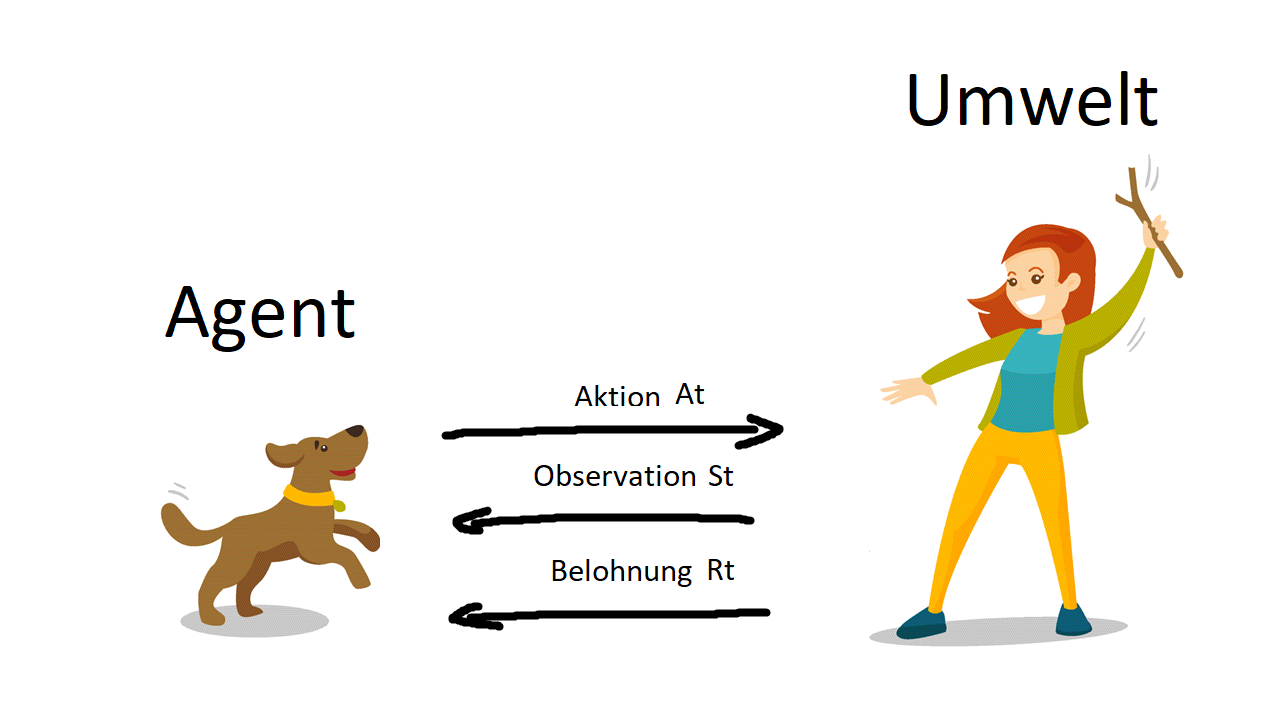
\includegraphics[scale=0.6]{pics/reinforcementLearningConcept.png}
    \caption{Veranschaulichung bestärkendes Lernen}
    \label{tech:fig:reinfconcept}
\end{figure}

OpenAI Gym hat also einen mehr oder weniger vorgegebenen Bauplan, und vorgegebene Regeln, nach welchen
so eine Künstliche Intelligenz aufgebaut werden muss. \\
Weitere, weit verbreitete Formen von machine learning sind supervised und unsupervised learning.
% Auf diese wird nur weiter eingegangen, wenn zu wenig Text für eine positive Note für die Diplomarbeit vorliegen sollte.

\subsection{Künstliche Intelligenz allgemein [H]}\label{tech:ki:head}
Künstliche Intelligenz funktioniert im Grunde genommen wie das menschliche Gehirn. Es basiert genauso auf Neuronen und deren Axonen, Dendriten und Terminale. Obwohl es verschiedene Arten von Neuronen gibt, haben sie alle gemeinsam, dass sie einen elektrischen Impuls als Reaktion auf einen Input aussenden. Dieser Output hängt von dem Neuron, welches das chemische und elektrische Signal verarbeitet, ab.

\begin{figure}[H]
    \centering
    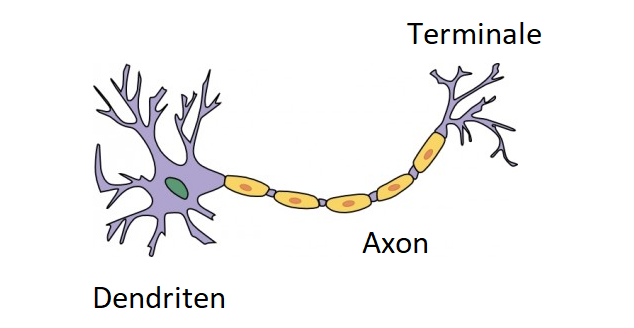
\includegraphics[scale=1]{pics/Neuron.png}
    \caption{Neuron}
    \label{fig:tech:Neuron}
\end{figure}

Genauso funktioniert auch ein Neuronales Netz. Auf eine Eingabe folgt über eine Verarbeitung der Eingabe eine Ausgabe. Und genau wie bei einem Menschen, welcher etwas Neues kennenlernt, weiß auch das Neuronale Netz nicht, was die korrekte Antwort auf ein Problem ist. Es muss sich also an die Lösung herantasten.

\begin{figure}[H]
    \centering
    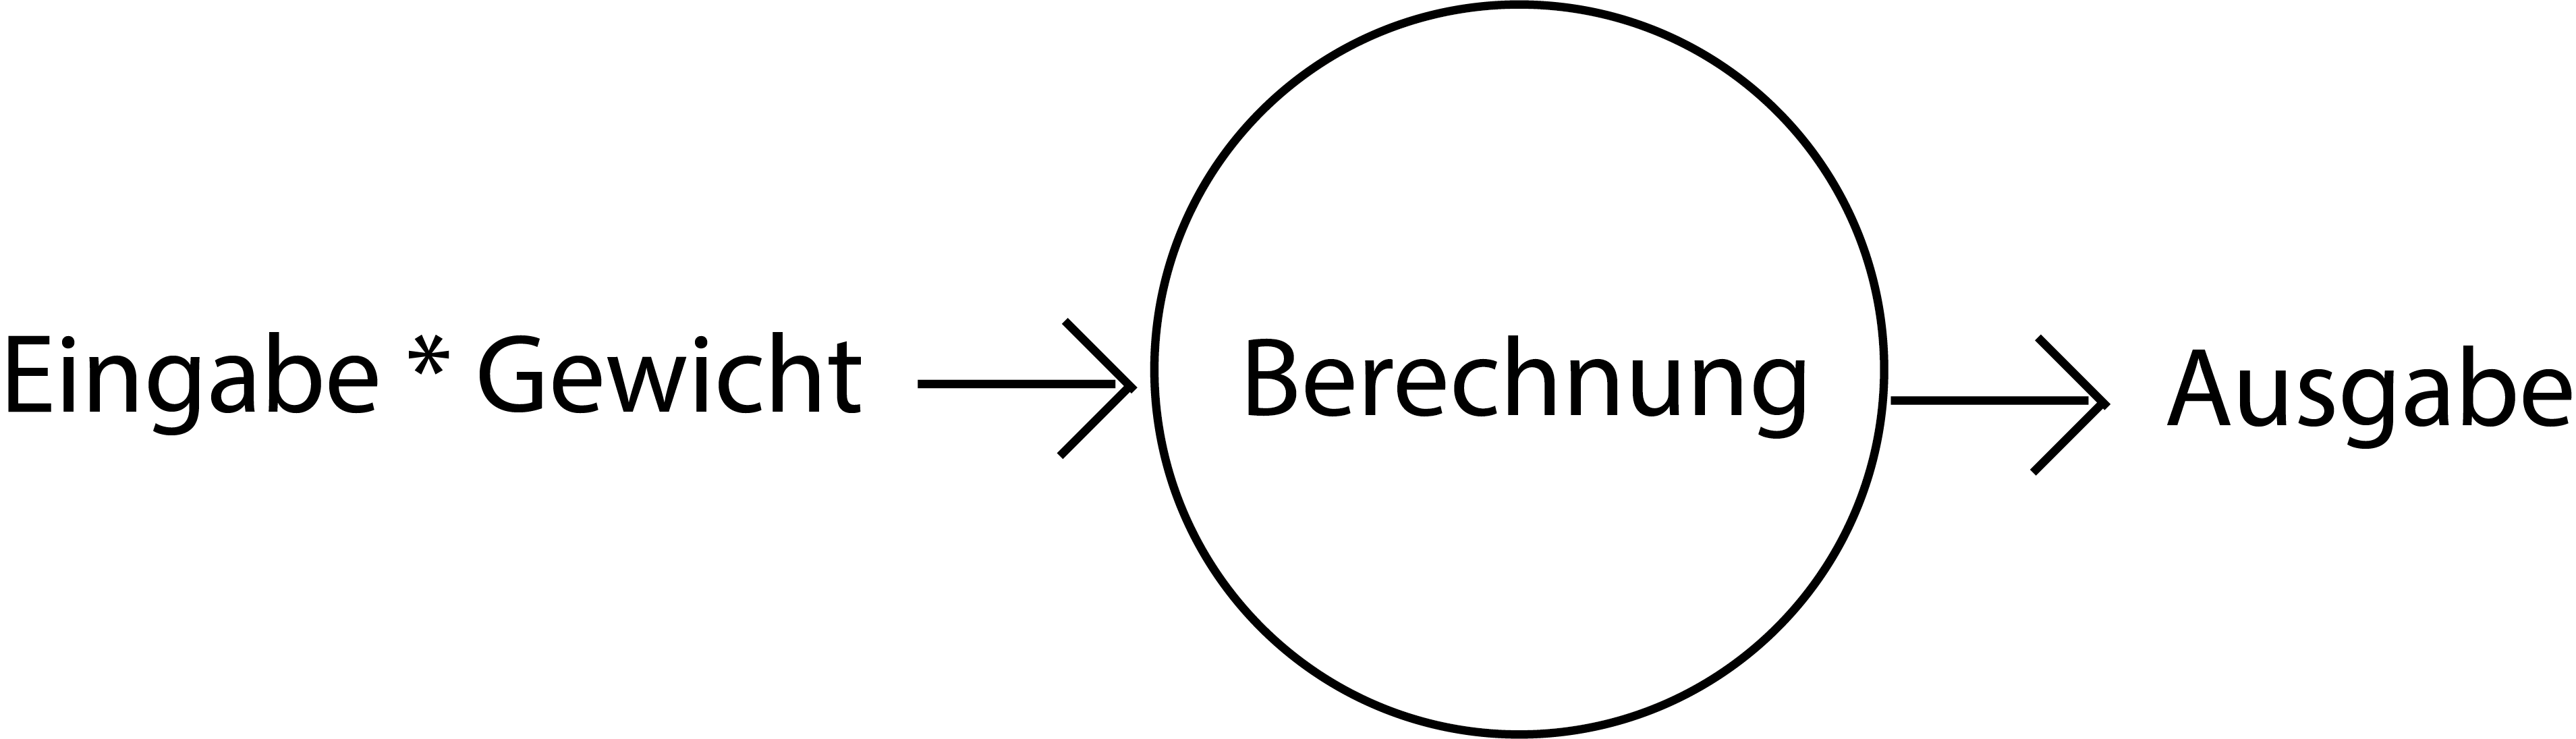
\includegraphics[scale=1]{pics/eba.png}
    \caption{Eingabe $\rightarrow$ Berechnung $\rightarrow$ Ausgabe}
    \label{fig:tech:eba}
\end{figure}

Ein einfaches mathematisches Beispiel hierfür wäre, wenn man einen einfachen Faktor mit zwei Nachkommastellen herausfinden möchte. Beispiel: Euro in USD umrechnen. Hierfür ist ein Faktor kleiner 1 nötig. Bevor der ganze Prozess des Lernens startet, muss man mit einer Eingabe starten. Dies ist zum Beispiel die Zahl 1. Somit erkläre ich der künstlichen Intelligenz im übertragenen Sinne: ``Bitte errechne mir wie viele USD in meiner Hand liegen.''. Es wurde also ein Input für die KI gefunden. Dieser Input wird über eine nicht ganz zufällig gewählte Gewichtung in eine Berechnung umgewandelt. Nehmen wir an, diese Gewichtung sei ein Faktor <1 also 0,99. ``Nicht ganz zufällig gewählt'', weil der Anwender, welcher die KI schreibt im Vorhinein schon wusste, dass ein USD weniger Wert ist, als ein Euro; der genaue Wert war jedoch unbekannt. Nach dieser Berechnung kommt ein Wert raus – nämlich 0.99 – welcher falsch ist. Damit die Künstliche Intelligenz jedoch weiß, ob sie richtig oder falsch rechnet, muss sie ein Feedback bekommen. Das heißt, dass der errechnete Wert und die Abweichung vom tatsächlichen Ergebnis (wenn dieses bekannt ist) zurückgegeben wird. In den meisten Fällen ist das Ergebnis bei präparierten Daten bereits bekannt, da diese als Trainingsdaten agieren. Wenn die Künstliche Intelligenz jedoch selbst Entscheidungen vorhersagen muss, muss diese bereits mit solchen Daten trainiert worden sein, um ein akkurates Ergebnis liefern zu können. In dieser Phase lernt sie jedoch auch nicht mehr dazu. Sind die Ergebnisse unbekannt, kann zum Beispiel das zuvor erklärte Reinforcement Learning als Lernstrategie herangezogen werden. Diese Abweichung wird nun mit einer weiteren Berechnung rückpropagiert und die Gewichte werden aktualisiert. Dieses Prozedere (Eingabe $\rightarrow$ Berechnung $\rightarrow$ Ausgabe $\rightarrow$ Fehler $\rightarrow$ Fehler rückpropagieren $\rightarrow$ Gewichte anpassen) wird so oft mit weiteren Trainingsdaten wiederholt, bis die KI einen minimalen Fehler (Differenz zwischen dem tatsächlichen Ergebnis und der Vorhersage) erreicht.
Allerdings können hier einige Faktoren zusätzliche beeinflusst werden, bevor die KI tatsächlich zu lernen beginnt, um ein maximal genaues Ergebnis zu erzielen. Beispielsweise beträgt der Wechselkurs von Euro zu USD 0,89. Also ein USD ist nur 0,89 so viel wert wie ein Euro. Wenn man es der KI ermöglicht, sich nur in zehntel-Schritten an die Lösung anzupassen, so passiert folgendes:
Die KI wird das tatsächliche Ergebnis von 0,89 nie erreichen. Die von der KI errechnete Lösung beträgt entweder 0,9 oder 0,8. Wenn man diesen Anpassungswert jedoch kleiner ansetzt, auf ein Hundertstel zum Beispiel, so wird diese den Wert zwar langsamer erreichen, jedoch wird er genau dem Ziel entsprechen.
Dieser Wert darf jedoch auch nie zu klein gewählt werden. Schaut man sich das an einem etwas komplexeren Beispiel an, so ist klar zu erkennen, dass in der folgenden Kurve der tatsächliche minimale Fehler nie erreicht wird. Um dies zu vermeiden, gibt es verschiedene Methoden. Als Exempel kann eine Art Fehler-Abtastungs-Beschleunigung herangezogen werden. Hier wird der Faktor, um welchen die Abweichung korrigiert wird, in einer Art Beschleunigung angepasst. Es muss sich also den aktuellen Wert wie einen Ball vorgestellt werden, welcher über einen Berg hinunterrollt.

\begin{figure}[H]
    \centering
    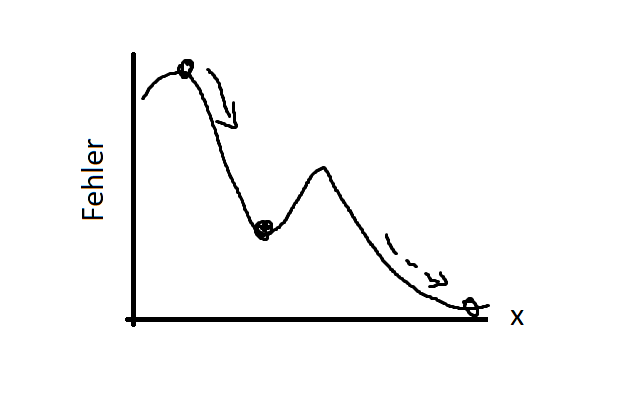
\includegraphics[scale=1]{pics/fehler.png}
    \caption{Fehlerkurve}
    \label{fig:tech:Fehler}
\end{figure}

Durch das Momentum kann der Ball nachfolgende Hindernisse überwinden. Die Gefahr dabei besteht jedoch, dass der Ball, wenn er nicht noch einmal angeschubst wird, in einem höheren Tal zum Stehen kommt, weil das Momentum zum Zurück- oder Weiterkommen fehlt. Es kann aber auch sein, dass der Ball nie genug Momentum hatte, da er zu wenig stark losbewegt wurde. All das und VIELES mehr fällt unter dem Begriff ``Hyperparameter Tuning''. Es muss also schon zu Beginn, bevor das Neuronale Netz überhaupt zu lernen beginnt, darauf geachtet werden, dass die Parameter stimmen, damit das Ergebnis einer perfekten Lösung am ähnlichsten ist.
Auch bei der Auswahl der Trainingsdaten ist enorme Vorsicht geboten. So ist es in einem amerikanischen Experiment dazu gekommen, dass eine Künstliche Intelligenz rassistisch wurde. Diese Software sollte Richtern dabei helfen, Häftlinge nach ihrer Entlassung zu beurteilen, wie hoch die Wahrscheinlichkeit sei, dass diese eine Wiederholungsstraftat begehen. Dabei kam heraus, dass dunkel-häutige Menschen weitaus gefährlicher eingestuft wurden als alle anderen. Das passierte nicht, weil diese tatsächlich eine höhere Gefahr darstellen, sondern weil in den USA dunkel-häutige Menschen öfter verhaftet werden. So stimmten auch die Proportionen in den für die KI vorliegenden Trainingsdatensätzen nicht. Daraufhin meinte ein beteiligter Journalist: „Künstliche Intelligenz hat keine Meinung oder ein Bewusstsein, sondern handelt nach dem, was wir ihr vorgeben. Diese Daten und Informationen sind oft ein Spiegel der Gesellschaft und reproduzieren so auch Vorurteile, zum Beispiel durch Über- und Unterrepräsentation“.
Zitat \textbf{Tobias Matzner}
% Quelle: https://www.rnd.de/wissen/wie-kuenstliche-intelligenz-rassismus-befoerdert-TZFL7KPOYRHFRBAA66OVOFS6QI.html%
\\
Und dass man mit Mathematik auch tatsächlich Spiele gewinnen kann, beziehungsweise, dass eine KI, welche immer wieder eine Gewichtung einer Eingabe aktualisiert, auch wirklich schlauer wird, wird im folgenden Beispiel erklärt. Hier geht es um ein Spiel in welchem man mit Mathematik eine Gewinnchance erhöht. Dies wird erzielt, indem man wiederholt Berechnungen ausführt und Gewichte aktualisiert. Somit wird die Gewinnchance in dem Spiel erhöht.
\\
Der Name des Spiels ist ``Hexapawn'' und wurde von \textit{Martin Gardner} entwickelt, welcher im Zweiten Weltkrieg half den ``Nazicode'' zu knacken.
\\
Das Spiel ist wie folgt aufgebaut: ein 3x3 Schachbrett bildet den Untergrund des Spiels. Auf den jeweils gegenüberliegenden Seiten befinden sich 3 Schachfiguren. Deutlich wird dies in der nachfolgenden Abbildung.


\begin{figure}[H]
    \centering
    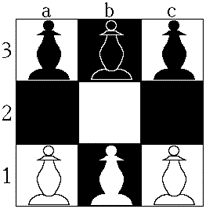
\includegraphics[scale=1]{pics/hexapawn/hexapawn_setup.png}
    \caption{Hexapawn Spielumgebung}
    \label{fig:tech:HexapawnSetup}
\end{figure}

Diese drei Figuren sind gleichwertig und dürfen sich Verhalten wie ein ``Bauer'' im Spiel Schach (also nur nach vor oder zum Schmeißen nach links und rechts). \textit{Martin Gardner} setzt dabei die Regel fest, dass der Mensch, auf welcher Seite er auch immer spielt, den ersten Zug macht. Somit ist der Mensch immer in den ungeraden Zügen dran (1, 3, 5, 7) und der Computer/die Künstliche Intelligenz/die Mathematik immer in den geraden Zügen (2, 4, 6) an der Reihe. Nach acht Zügen gibt es garantiert immer einen Gewinner. Das Ziel des Spiels ist es, dass man alle gegnerischen Figuren schmeißt.
\\
Um einen solchen ``Hexapawn''-Computer zu bauen braucht man vierundzwanzig Streichholzschachteln. Auf jeder dieser Streichholzschachteln sind alle möglichen ``Hexapawn''-Züge aufgezeichnet, und wie auf diese reagiert werden kann. Dies wird in der nachstehenden Grafik veranschaulicht. Seitlich haben diese Schachteln eine Öffnung.


\begin{figure}[H]
    \centering
    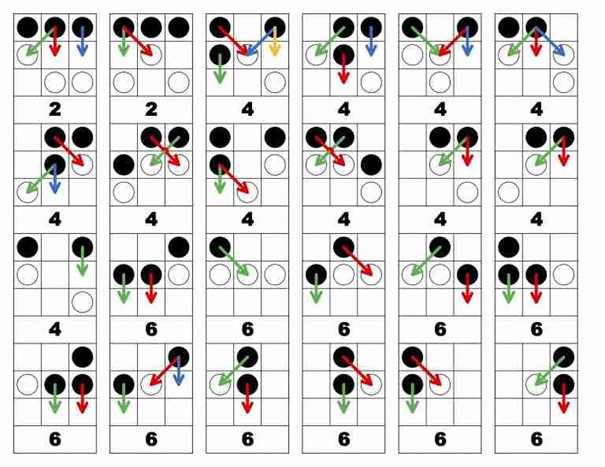
\includegraphics[scale=1]{pics/hexapawn/hexapawn_zuege.jpg}
    \caption{Hexapawn mögliche Züge}
    \label{fig:tech:HexapawnZuege}
\end{figure}


Wählt der Mensch und Gegner der Maschine den ersten Zug, so ist dieser garantiert auf einen der beiden ersten Abbildungen zu sehen. In den Zündholzschachteln befinden sich farbige Kugeln. Schüttelt man diese nun, und lässt eine Kugel aus der Öffnung seitlich fallen, so wählt man den Zug, bei welchem die Pfeilfarbe der Kugelfarbe entspricht. So spielt man das Spiel zu ende, bis es nach dem achten Zug einen garantierten Gewinner gibt und zieht dann ein Resultat. Das heißt, wenn die KI gewonnen hat, kann man die Gewinnchance bei einem nächsten Spiel erhöhen. Dies erreicht man, indem man alle farbigen Kugeln, welche aus der Streichholzschachtel fielen, doppelt zurücklegt. Wenn es also in der ersten Schachtel grün, rot und blau gibt und grün als erster Zug eines Spiels gewählt wurde, welches zu einem Sieg führte, so gibt man in die erste Schachtel eine zweite grüne Kugel. Somit wird die Wahrscheinlichkeit, dass man bei einem nächsten Spiel einen Zug wählt, welcher schon einmal zu einem Sieg führte, erhöht. Ähnlich kann man dies auch bei Zügen machen, welche dazu führten, das Spiel zu verlieren. Hier kann man die Wahrscheinlichkeit zu verlieren verringern, indem man die Farbige Kugel aus dem Spiel entnimmt.
\\
So hat \textit{Martin Gardner} bewiesen, dass man Spiele mit Mathematik gewinnen kann. Auf diesem Prinzip basieren auch viele andere Künstliche Intelligenzen. Natürlich können in dem Spiel ``Hexapawn'' binnen weniger Augenblicke alle möglichen Kombinationen errechnet werden und somit eine perfekte Spielstrategie entwickelt werden. Anders ist dies bei Spielen wie ``Schach'' oder ``GO''. Bei diesen Spielen gibt es unzählige Kombinationsmöglichkeiten, bei welchen es selbst für eine Maschine nahezu unmöglich ist, alle Spielkombinationen auszuprobieren. Jedoch ist es für einen Computer möglich in kürzester Zeit extrem viele Berechnungen durchzuführen. Ein tage-/monate-/jahrelanges Lernen in einer Geschwindigkeit, welche für Menschen unmöglich ist, führt für die KI also auch zu einer immer höheren Gewinnchance für jedes Spiel. Dadurch ist es für die sogenannte ``AlphaGo''-KI möglich gewesen selbst die besten Spieler der Welt im Spiel ``GO'' zu besiegen. Durch die vielen Kombinationsmöglichkeiten ist es trotzdem nicht gegeben, dass die KI pro Zug die perfekte Auswahl trifft. Jedoch werden immer Züge gewählt, welche in bisherigen Spielen zu der höchsten Gewinnchance führten. Somit ist es also auch für eine Maschine möglich, nicht deterministische Ereignisse mit einer gewissen Wahrscheinlichkeit, welche oft der realen Zukunft entspricht, vorherzusagen (Beispiel: Wettervorhersage).

\setauthor{Weinzierl Ben}
\newpage
\section{Photoshop [W]}
Für die Character Animation wurde Adobe Photoshop benutzt. Photoshop ist ein Programm mit dem 
im professionellen wie im Amateurbereich gearbeitet wird um Bilder zu bearbeiten. 
Aufgrund der unglaublich zahlreichen Einsatzbereiche und Funktionen von Photoshop ist es 
eines der beliebtesten Programme der Design- und Bildbearbeitungsbranche. 
Durch den großen Funktionsumfang ist Photoshop zwar sehr einsteigerunfreundlich, jedoch 
hat es sich trotzdem durchgesetzt. Mit ca. 90 Prozent Marktanteil ist es das mit Abstand größte
Bildbearbeitungsprogramm. Dadurch ist der Preis mit 24€ pro Monat für die Software sehr hoch, wobei dazugesagt werden muss,
dass laut einer Umfrage im Jahr 2007 ca. 58 Prozent der User und Userinnen das Programm als Schwarzkopie verwenden. 

Eine wichtige Funktion, welche bei dieser Arbeit viel verwendet wurde, ist das "Form erzeugen" Werkzeug. Ausgewählt wird es mit dem Shortcut "U". Damit können Formen erstellt und verändert werden. Um zum Beispiel ein Viereck zu erstellen, muss das Unterwerkzeug "Rechteck-Werkzeug" auswählen. Danach
kann eine beliebig große Fläche aufgezogen werden. 
\begin{figure}[H]
    \centering
    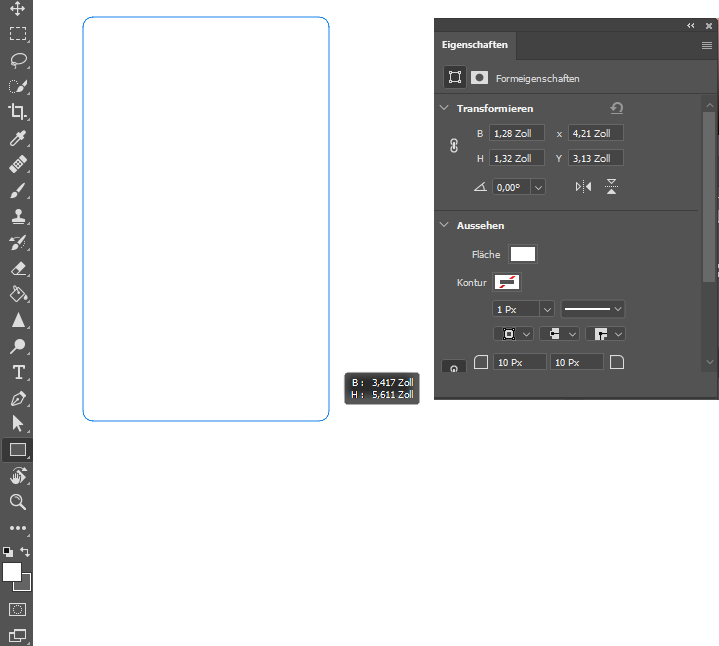
\includegraphics[scale=0.7]{pics/erzeugen.png}
    \caption{Erzeugen Werkzeug}
\end{figure}

Um die Formen in die richtige Position zu bekommen, wurde mit dem "Transformieren" Werkzeug
gearbeitet. Verwendet wird es unter dem Reiter "Bearbeiten -> Transformieren". 
Um die Fläche zu skalieren wird an den Ecken mit der Maus die Größe verändert. Sollen die Proportionen des Bildes erhalten bleiben
kann dabei die Umschalt-Taste gedrückt werden. Damit die Ebene gedreht werden kann, muss an den Rändern gehovert werden bis das Drehsymbol erscheint. 
Um die Ebene zu spiegeln oder auf den Kopf zu stellen kann der Befehl 'Horizontal Spiegeln' bzw. 'Um 180° drehen'.




